% Figures/data_distribution.tex
\begin{figure}[ht]
    \centering
    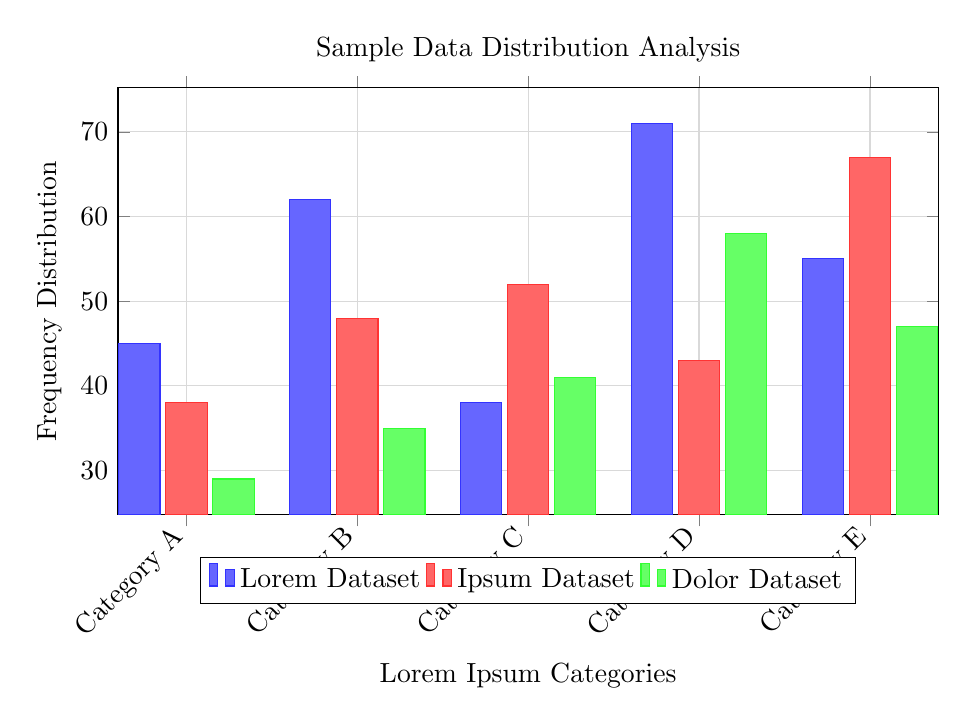
\begin{tikzpicture}
        \begin{axis}[
                width=12cm,
                height=7cm,
                xlabel={Lorem Ipsum Categories},
                ylabel={Frequency Distribution},
                title={Sample Data Distribution Analysis},
                ybar,
                bar width=15pt,
                enlarge x limits=0.1,
                legend style={at={(0.5,-0.1)}, anchor=north, legend columns=-1},
                symbolic x coords={Category A, Category B, Category C, Category D, Category E},
                xtick=data,
                x tick label style={rotate=45, anchor=east},
                grid=major,
                grid style={gray!30},
            ]

            % Dataset 1
            \addplot[fill=blue!60, draw=blue!80] coordinates {
                    (Category A, 45)
                    (Category B, 62)
                    (Category C, 38)
                    (Category D, 71)
                    (Category E, 55)
                };
            \addlegendentry{Lorem Dataset}

            % Dataset 2
            \addplot[fill=red!60, draw=red!80] coordinates {
                    (Category A, 38)
                    (Category B, 48)
                    (Category C, 52)
                    (Category D, 43)
                    (Category E, 67)
                };
            \addlegendentry{Ipsum Dataset}

            % Dataset 3
            \addplot[fill=green!60, draw=green!80] coordinates {
                    (Category A, 29)
                    (Category B, 35)
                    (Category C, 41)
                    (Category D, 58)
                    (Category E, 47)
                };
            \addlegendentry{Dolor Dataset}

        \end{axis}
    \end{tikzpicture}
    \caption{Lorem ipsum dolor sit amet distribution showing comparative analysis across different categorical variables in the study dataset.}
    \label{fig:data_distribution}
\end{figure}